\documentclass{standalone}

\usepackage{tikz}
\usetikzlibrary{calc}
\newsavebox\mybox

\begin{document}
% Diagram of the TeX box model and its dimensions
% Copyright (C) 2001 by Martin Scharrer <martin@scharrer.me>, Nov 12th 2011
% This is free code under the LPPL v1.3 or later version OR the CC BY-SA 3.0
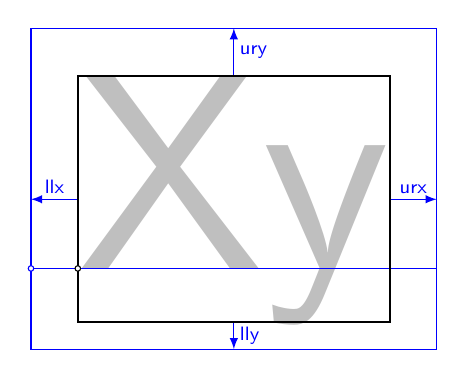
\begin{tikzpicture}[font=\sffamily,>=latex]
   % Save example text in box
   \def\text{\scalebox{10}{Xy}}
   \sbox\mybox{\pgfinterruptpicture\sffamily\color{black!25}\scalebox{10}{Xy}\endpgfinterruptpicture}
   \def\HEIGHT{\ht\mybox}
   \def\WIDTH{\wd\mybox}
   \def\DEPTH{\dp\mybox}
   \def\LLX{.15\WIDTH}
   \def\LLY{.5\DEPTH}
   \def\URX{.15\WIDTH}
   \def\URY{.25\HEIGHT}
   % Text node:
   \node [inner sep=0pt,anchor=base west] {\usebox\mybox};
   % Baseline
   \draw (0,0) -- (\WIDTH,0);% node [above,midway] {baseline};
   %\draw [<-,shorten <=2pt] (0,0) -- (2ex,-2ex) -- +(.5ex,0) node [right=-0.5ex] {origin};
   % Dimensions
   \begin{scope}[blue,every node/.append style={inner sep=2pt}]
    \begin{scope}
        \draw ([shift={(-\LLX,-\LLY)}]0,-\DEPTH) rectangle ([shift={(\URX,\URY)}]\WIDTH,\HEIGHT);
       %\node [inner sep=0pt,anchor=base west,semitransparent,color=blue] {\text};
    \end{scope}
   %\draw [->,.!45] (\WIDTH,\HEIGHT) -- ++(-\URX,-\URY);
   %\draw [->,.!45] (0,-\DEPTH) -- ++(\LLX,\LLY);
    \draw [->] (.5\WIDTH,-\DEPTH) -- ++(0,-\LLY) node [right,midway] {\scriptsize lly};
    \draw [->] (0,.5*\HEIGHT-.5*\DEPTH) -- ++(-\LLX,0) node [above,midway] {\scriptsize llx};
    \draw (-\LLX,0) -- ([shift={(+\URX,0)}]\WIDTH,0);
    \draw [->] (.5\WIDTH,\HEIGHT) -- ++(0,\URY) node [right,midway] {\scriptsize ury};
    \draw [->] (\WIDTH,.5*\HEIGHT-.5*\DEPTH) -- ++(\URX,0) node [above,midway] {\scriptsize urx};
    \path [fill=white,draw] (-\LLX,0) circle (1pt);
   \end{scope}
   % Box
   \draw [thick] (0,-\DEPTH) rectangle (\WIDTH,\HEIGHT);
   % Origin
   \path [fill=white,draw=black] (0,0) circle (1pt);
   % Center inner box
   \path let
        \p1 = (current bounding box.south west),
        \p2 = (current bounding box.north east),
        \p3 = (0,-\DEPTH),
        \p4 = (\WIDTH,\HEIGHT)
   in
        (\x3-\x2+\x4,\y3) rectangle (\x4+\x3-\x1,\y4);
\end{tikzpicture}
\end{document}
